\documentclass{article}%
\usepackage[T1]{fontenc}%
\usepackage[utf8]{inputenc}%
\usepackage{lmodern}%
\usepackage{textcomp}%
\usepackage{lastpage}%
\usepackage{graphicx}%
%
\title{Chronic Morphine Treatment Attenuates Cell Growth of Human BT474 Breast Cancer Cells by Rearrangement of the ErbB Signalling Network}%
\author{\textit{Wallace Morgan}}%
\date{04-17-2008}%
%
\begin{document}%
\normalsize%
\maketitle%
\section{Specialized neonatal health workers at our Center for Advanced Neonatal Health are working on the science behind how the key component of functional kidney disease is activated when embryonic cells respond to molecules of the human telomeres}%
\label{sec:SpecializedneonatalhealthworkersatourCenterforAdvancedNeonatalHealthareworkingonthesciencebehindhowthekeycomponentoffunctionalkidneydiseaseisactivatedwhenembryoniccellsrespondtomoleculesofthehumantelomeres}%
Specialized neonatal health workers at our Center for Advanced Neonatal Health are working on the science behind how the key component of functional kidney disease is activated when embryonic cells respond to molecules of the human telomeres.\newline%
The Link conference is being held in Denver, Colorado, May 3{-}8, 2008.\newline%
Co{-}organizer Elizabeth L. Monahan{-}McDowell, Ph.D., of the Center for Advanced Neonatal Health, is a pioneer in neonatal medical research and University of Oregon pediatric medical professor at LifeCam and co{-}author of a study that will be presented in the 2008 Contents of the Health Department meeting. L. Monahan{-}McDowell has been working on and writing about the link between these molecules and fundamental structures in the human telomeres since 1995. Her research interests include translating, repairing and monitoring the genetic status of progenitor cells; controlling cell migration; and genetics. She has developed and written more than 20 articles and directories on neonatal health. L. Monahan{-}McDowell is the founder and director of Neonatal Med Injury Research and Association of Neonatal Health Professionals.\newline%
The Link conference is sponsored by the Center for Advanced Neonatal Health.\newline%
This article was prepared by Sarah S. Harman, M.D., M.P.H., assistant professor of medicine and microbiology at Hopkins Medical School and a specialist in neonatal medicine. A previous article on the link between progenitor cells and tissues was co{-}authored by S. Harman and Seema Tsipras, M.D., director of the J. Peregrine Genetics Clinical Research Center at the Medical University of America.\newline%
Source:\newline%
Christine Raff, Ph.D., professor of neonatal medicine at the University of Oregon\newline%

%


\begin{figure}[h!]%
\centering%
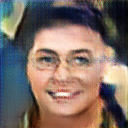
\includegraphics[width=120px]{./photos_from_epoch_8/samples_8_228.png}%
\caption{a man wearing a tie and a hat .}%
\end{figure}

%
\end{document}